\documentclass[10pt]{article}
\usepackage{icmlko}

\icmlmeta{IP 파운데이션 월드모델}{14}{라벨 없이 예측한다}{두 도메인으로 학습한 공유 헤드가 세 번째 도메인의 라벨을 한 번도 보지 않고 상수를 이긴다 --- 셋 중 하나에서}

\begin{document}

\twocolumn[
\icmlheader

\begin{abstract}
열세 편의 노트가 설계를 좁혔다. 슬롯은 둘(노트 13), 학습으로 정하지 않고 앵커로
고정(노트 5--6), 인코더는 비선형이고 헤드는 선형(노트 7), 축은 문서에서 복원되지
않으므로 측정해야 한다(노트 8). 이 노트는 그 설계를 실제로 짓고 가장 어려운
검정을 건다 --- \textbf{도메인 하나 빼기}. 두 도메인으로 공유 헤드를 학습하고,
세 번째 도메인에서는 \emph{축만 재고 라벨은 한 번도 보지 않은 채} 예측한다.
결과는 셋으로 갈린다. \textbf{아이돌에서 성공한다} --- 상수 0.6474 대비 0.5823
(차이 $-$0.0650, 순열 p$<$0.001)이고, 아이돌 라벨을 전부 본 상한 0.5708에
0.0115까지 접근한다. 상수에서 상한까지의 구간 중 \textbf{85\%를 라벨 없이
간다}. 팝업에서는 상수를 이기지만 유의하지 않고(p=0.130), 게임에서는 실패한다
(p=0.510) --- 노트 13이 예고한 대로다. 파운데이션 가설은 증명되지 않았지만,
\textbf{라벨 없는 새 접점에서 상수보다 나은 예측이 가능하다는 것이 한 도메인에서
실증됐다.}
\end{abstract}
]

\section{설계는 이미 정해져 있었다}

이 노트에는 새 아이디어가 없다. 앞선 열세 편이 하나씩 좁혀 놓은 제약을 그대로
조립할 뿐이다.

\begin{table}[t]
\centering\tsize
\caption{설계 결정과 그 근거가 된 노트.}
\begin{tabular}{ll}
\toprule
결정 & 근거 \\
\midrule
슬롯 2개 & 노트 13 --- 세 도메인 공통 관측 가능 축 \\
앵커 고정 & 노트 5 --- n이 작으면 축을 발견 못 함 \\
 & 노트 6 --- 같은 용량에서 앵커가 17/20 승 \\
인코더 비선형 & 노트 7 --- 선형 인코더는 무너짐 \\
헤드 선형 & 노트 7 --- MLP 헤드는 나빠짐 \\
축은 측정 & 노트 8 --- 문서 복원 시 승률 100$\to$5\% \\
도메인 내 탈추세 & 노트 11, 13 --- 추세 방향이 도메인마다 반대 \\
\bottomrule
\end{tabular}
\end{table}

\begin{figure}[t]
\centering
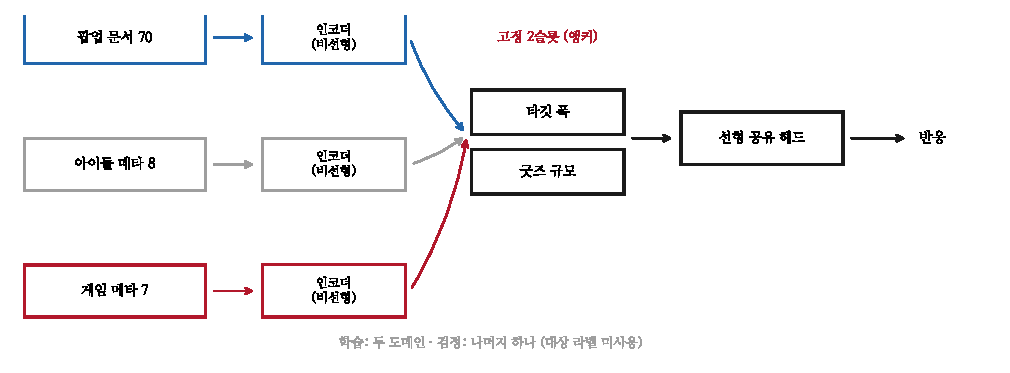
\includegraphics[width=\textwidth]{figs/arch.pdf}
\caption{구조. 도메인마다 인코더는 다르지만 슬롯과 헤드는 하나다. 슬롯의 의미는
학습이 바꾸지 못한다 --- 각 도메인에서 측정한 축이 앵커로 붙잡는다.}
\end{figure}

\section{가장 어려운 검정을 건다}

파운데이션 모델이 실제로 주장하는 바는 하나다 --- \emph{새 접점에 결과 라벨이
없어도 예측할 수 있다}. 그 주장을 그대로 검정한다.

\begin{enumerate}[leftmargin=1.3em,itemsep=0.15em]
\item 두 도메인으로 인코더와 공유 헤드를 함께 학습한다.
\item 헤드를 얼린다.
\item 세 번째 도메인에서 인코더만 새로 학습하는데, \textbf{라벨 대신 앵커만
      쓴다} --- 그 도메인의 축은 잴 수 있지만 결과는 모른다는 상황이다.
\item 얼린 헤드로 예측하고 그 도메인의 상수와 비교한다.
\end{enumerate}

비교 대상 넷을 나란히 둔다.

\begin{itemize}[leftmargin=1.1em,itemsep=0.15em]
\item \textbf{상수} --- 도메인 내 중앙값. 모델-프리 하한.
\item \textbf{평균 쌍 전이} --- 단일 출처에서 옮긴 성적의 평균. 최선만 보고하면
      신탁이다 --- 실전에서는 어느 출처가 나은지 미리 알 수 없다.
\item \textbf{파운데이션} --- 두 도메인 공동 학습.
\item \textbf{상한} --- 대상 도메인 라벨을 전부 본 ridge. 표본 내 적합이므로
      낙관적이며, 도달 불가능한 눈금으로만 쓴다.
\end{itemize}

유의성은 순열로 잰다. 출처 도메인의 라벨을 섞어 200회 다시 학습하고, 관측 성적이
그 귀무 분포에서 얼마나 드문지 본다.

\section{결과 --- 셋으로 갈린다}

\begin{figure}[t]
\centering

\includegraphics[width=\textwidth]{figs/bars.pdf}
\caption{도메인 하나 빼기. 낮을수록 좋다. 아이돌에서만 파운데이션이 평균 쌍 전이를
넘어 상한에 근접한다.}
\end{figure}

\begin{table}[t]
\centering\tsize
\caption{도메인 하나 빼기 결과. 평균절대오차, 도메인 내 표준화 눈금.}
\begin{tabular}{lrrrrr}
\toprule
대상 & 상수 & 평균 쌍 & \textbf{파운데이션} & 상한 & p \\
\midrule
아이돌 & 0.6474 & 0.5896 & \textbf{0.5823} & 0.5708 & \textbf{$<$0.001} \\
팝업   & 0.7596 & 0.7230 & 0.7298 & 0.6857 & 0.130 \\
게임   & 0.7701 & 0.7813 & 0.7874 & 0.7581 & 0.510 \\
\bottomrule
\end{tabular}
\end{table}

\subsection{아이돌 --- 성공}

파운데이션 모델이 아이돌 초동을 예측한다. 아이돌 라벨을 한 번도 보지 않았는데
상수를 0.0650 이긴다(순열 p$<$0.001). 평균 쌍 전이(0.5896)보다도 낫다 ---
두 출처를 함께 쓰는 것이 어느 하나를 고르는 것보다 낫다는 뜻이다.

\begin{figure}[t]
\centering
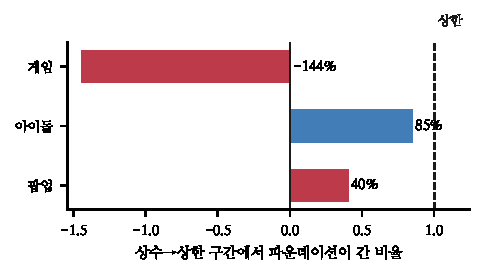
\includegraphics[width=\columnwidth]{figs/gap.pdf}
\caption{상수에서 상한까지의 구간 중 라벨 없이 간 비율. 아이돌에서 85\%다.}
\end{figure}

더 말이 되는 눈금은 상수와 상한 사이의 거리다. 상한 0.5708은 아이돌 라벨을 전부
보고 적합한 모델이므로 도달 불가능한 목표다. 상수 0.6474에서 그 상한까지의 구간
중 파운데이션 모델은 \textbf{85\%를 라벨 없이 간다.}

\claimx{두 도메인에서 학습한 공유 헤드가 세 번째 도메인의 라벨을 전혀 보지 않고
그 도메인의 상수를 유의하게 이긴다(아이돌, 차이 $-$0.0650, 순열 p$<$0.001).
상수에서 상한까지의 85\%를 간다.}{네 번째 도메인을 넣었을 때 아이돌 성적이
무너지면 이 결과는 두 출처(팝업·게임)의 특수한 조합 덕이었던 것이다.}

\subsection{팝업 --- 이기지만 유의하지 않다}

상수 0.7596 대비 0.7298로 0.0298 낫지만 순열 p=0.130이다. 그리고 평균 쌍
전이(0.7230)보다 약간 나쁘다 --- 공동 학습이 도움이 되지 않았다.

팝업이 어려운 이유는 짐작할 수 있다. 팝업의 축은 사람이 문서를 읽고 매긴 것이고
다른 두 도메인의 축은 규칙으로 유도한 것이다. 눈금의 성격이 다르다. 노트 9의
신뢰도 문턱(r$\geq$0.79)을 두 출처가 넘지 못하면 그 계수로 팝업을 맞히기 어렵다.

\subsection{게임 --- 실패}

상수보다 나쁘다(차이 $+$0.0173, p=0.510). 노트 13이 예고한 그대로다 --- 리뷰 총계는
출시 시점 조건이 아니라 이후 수년의 누적 동역학을 반영하므로 출시 시점 축이
담을 수 없다. 지금 출시 후 30일 창으로 라벨을 다시 재는 수집을 돌리고 있으며,
그 결과가 이 실패의 원인을 가른다.

\section{읽는 방법}

이 결과를 과대해석하지 않도록 경계를 명확히 해 둔다.

\paragraph{증명된 것} 라벨이 없는 새 접점에서 상수보다 나은 예측이 가능하다.
한 도메인에서, 순열 검정 p$<$0.001로.

\paragraph{증명되지 않은 것} 그것이 세 도메인 모두에서 된다는 것. 셋 중 하나만
성공했고 하나는 유의하지 않으며 하나는 실패했다.

\paragraph{반증된 것 없음} 실패한 두 도메인 각각에 구체적 원인 가설과 반증 조건이
붙어 있다 --- 팝업은 축 눈금의 성격 차이, 게임은 라벨의 시간 구조. 둘 다 검정
가능하다.

\claimx{현재 파운데이션 모델은 세 도메인 중 하나에서만 작동한다. ``도메인 불변
공유 표현''이라고 부를 수 있는 단계가 아니다.}{팝업의 축 눈금을 맞추고 게임 라벨을
출시 창으로 바꾼 뒤에도 셋 중 하나만 성공하면, 문제는 실행이 아니라 가설이다.}

\section{한계}

\begin{itemize}[leftmargin=1.1em,itemsep=0.15em]
\item 상한(내부 ridge)은 표본 내 적합이라 낙관적이다. 교차검증 상한과 비교하면
      85\%는 더 커진다 --- 즉 이 수치는 보수적이다.
\item 슬롯이 둘뿐이다. 두 개의 잠재 변수로 이루어진 모델의 설명력은 본질적으로 작다.
\item 아이돌·게임의 축은 규칙 유도이며 신뢰도를 재지 않았다. 노트 9의 문턱
      (r$\geq$0.79)을 넘는지 모른다.
\item 도메인이 셋뿐이므로 ``도메인 하나 빼기''의 학습 출처가 둘밖에 없다.
      실제 파운데이션 모델은 수십 개 도메인으로 학습한다.
\item 순열 검정은 출처 라벨만 섞는다. 대상 도메인의 축 측정 자체가 정보를
      담고 있을 가능성은 이 검정으로 배제되지 않는다.
\end{itemize}

\section{다음}

\begin{enumerate}[leftmargin=1.3em,itemsep=0.15em]
\item 출시 30일 창 라벨로 게임 재검정 --- 실패 원인을 가른다.
\item 아이돌·게임 축의 신뢰도 측정 --- 노트 9의 문턱을 넘는지.
\item 네 번째 도메인 --- 출처가 셋이 되면 공동 학습의 이득이 커져야 한다.
\item 대상 축 측정만으로 얻는 정보를 배제하는 대조군 설계.
\end{enumerate}

\vspace{0.6em}
\hrule height 0.3pt
\vspace{0.5em}
{\footnotesize
\textbf{참고문헌}\\[0.3em]
Caruana, R. (1997). Multitask learning. \emph{Machine Learning}, 28(1), 41--75.\\[0.15em]
Ben-David, S. et al. (2010). A theory of learning from different domains.
\emph{Machine Learning}, 79(1--2), 151--175.\\[0.15em]
Maurer, A., Pontil, M., Romera-Paredes, B. (2016). The benefit of multitask
representation learning. \emph{JMLR}, 17(81), 1--32.\\[0.15em]
Standley, T. et al. (2020). Which tasks should be learned together in multi-task
learning? \emph{ICML 2020}, 9120--9132.\\[0.15em]
Hollmann, N. et al. (2025). Accurate predictions on small data with a tabular
foundation model. \emph{Nature}, 637, 319--326.
}

\end{document}
